% sections/02_intro.tex

\section{Introduction \& Motivation}

% --- SLIDE 1: The Pipeline (Full Width Visual) ---
\begin{frame}{The Market Basket Problem: From Paper to Patterns}
    \centering
    \begin{tikzpicture}[scale=1.1, every node/.style={transform shape}]
        % --- STAGE 1: Physical Data ---
        \node[font=\bfseries\small, gray] at (1.4, 6.2) {1. Physical Transactions};
        \draw[thick, fill=white] (0,2) rectangle (2.8,5.8);
        \draw[thick] (0,2) -- (0.2,1.8) -- (0.4,2) -- (0.6,1.8) -- (0.8,2) -- (1.0,1.8) -- (1.2,2) -- (1.4,1.8) -- (1.6,2) -- (1.8,1.8) -- (2.0,2) -- (2.2,1.8) -- (2.4,2) -- (2.6,1.8) -- (2.8,1.8) -- (2.8,2);
        
        \node at (1.4, 5.4) {\textbf{\tiny RECEIPT}};
        \node[anchor=west] at (0.1, 4.8) {\tiny MILK ........ \$2.5};
        \node[anchor=west] at (0.1, 4.4) {\tiny BREAD ..... \$1.8};
        \node[anchor=west] at (0.1, 4.0) {\tiny BEER ........ \$12};
        \node[anchor=west] at (0.1, 3.6) {\tiny DIAPERS .. \$25};
        
        % --- Transition Arrow 1 ---
        \draw[->, ultra thick, gray!30] (3.0, 3.8) -- (4.0, 3.8) node[midway, above, font=\tiny\itshape, text=gray] {Digitize};

        % --- STAGE 2: Digital Representation ---
        \node[font=\bfseries\small, PrimaryColor] at (6.0, 6.2) {2. Digital "Baskets"};
        \draw[thick, rounded corners, fill=PrimaryColor!5] (4.2, 2.3) rectangle (7.8, 5.3);
        
        \node[draw, fill=PrimaryColor!20, inner sep=2pt] at (6.0, 4.3) {\tiny T1: \{Milk, Bread, Beer, Diapers\}};
        \node[draw, fill=white, inner sep=2pt] at (6.0, 3.6) {\tiny T2: \{Milk, Eggs, Bread\}};
        \node[draw, fill=white, inner sep=2pt] at (6.0, 2.9) {\tiny T3: \{Beer, Diapers, Chips\}};
        \node at (6.0, 2.5) {\tiny $\vdots$};

        % --- Transition Arrow 2 ---
        \draw[->, ultra thick, SecondaryColor] (6.0, 2.1) -- (6.0, 0.5);
        
        % --- STAGE 3: Knowledge Discovery ---
        \node[below, SecondaryColor, font=\bfseries] at (6.0, 0.5) {3. Discover Frequent Itemsets};
        \node[below, font=\scriptsize, text=gray] at (6.0, 0.1) {Search Space: $2^n$ Subsets};
    \end{tikzpicture}
\end{frame}

% --- SLIDE 2: Simple Examples & Goal ---
\begin{frame}{Mining Actionable Patterns}
    \textbf{Examples of Association Rules:}
    \vspace{0.3cm}
    \begin{itemize}
        \item \small $\{Milk, Bread\} \implies \{Eggs\}$
        \item \small $\{Beer\} \implies \{Diapers\}$
        \item \small $\{Wine\} \implies \{Cheese\}$
        \item \small $\{Laptop\} \implies \{Mouse, Keyboard\}$
    \end{itemize}

    \vfill

    \begin{alertblock}{The Data Mining Goal}
        \centering \textbf{Find all subsets of items (itemsets) that appear in at least $s$ transactions within a massive dataset.}
    \end{alertblock}
    
    \vspace{0.4cm}
    \begin{itemize}
        \item \small \textbf{Applications:} Cross-selling, inventory management, and store layout optimization.
    \end{itemize}
\end{frame}

% --- SLIDE 3: The Technical Challenge ---
\begin{frame}{The Technical Challenge: Complexity}
    \begin{columns}[T, onlytextwidth]
        \begin{column}{0.60\textwidth}
            \centering
            \begin{tikzpicture}[scale=0.8]
                % Axes
                \draw[->, thick] (0,0) -- (5,0) node[right, font=\tiny] {Items ($n$)};
                \draw[->, thick] (0,0) -- (0,4) node[above, font=\tiny] {Complexity};
                
                % Linear Curve O(n)
                \draw[thick, gray!60] (0,0) -- (4,1) node[right, font=\tiny] {$O(n)$};
                
                % Exponential Curve O(2^n)
                \draw[ultra thick, SecondaryColor] (0,0.1) .. controls (2,0.2) and (3,0.5) .. (4.2,3.8) 
                    node[left, font=\tiny, xshift=-2pt] {$O(2^n)$};
                
                % Explosion Marker
                \draw[dashed, red] (3.2,0) -- (3.2,1.2);
                \node[red, font=\tiny\bfseries, anchor=west] at (3.2, 0.8) {Explosion!};
                
                % Annotations
                \node[fill=white, draw=gray!30, rounded corners, font=\tiny, inner sep=2pt] at (2,3) {Brute Force fails at $n > 50$};
            \end{tikzpicture}
            
            \vspace{0.4cm}
            \scriptsize
            $n=100 \implies 2^{100}$ subsets. \\
            $\approx 3,000\times$ Age of Universe by Brute Force.
        \end{column}

        \begin{column}{0.38\textwidth}
            \centering
            \begin{minipage}{\textwidth}
                \centering
                \textbf{Power Set for $n=4$} \\
                \vspace{0.1cm}
                \renewcommand{\arraystretch}{1.1}
                \scriptsize
                \begin{tabular}{l l}
                    \hline
                    \textbf{Size} & \textbf{Subsets} \\ \hline
                    $k=0$ & $\emptyset$ \\
                    $k=1$ & $\{a\}, \{b\}, \{c\}, \{d\}$ \\
                    $k=2$ & $\{ab\}, \{ac\}, \{ad\}, \dots$ \\
                    $k=3$ & $\{abc\}, \{abd\}, \dots$ \\ 
                    $k=4$ & $\{abcd\}$ \\ \hline
                \end{tabular}
                \vspace{0.2cm}
                \small \textbf{Total: 16 Combinations} \\
                \scriptsize \textit{Adding 1 item doubles the work!}
            \end{minipage}
        \end{column}
    \end{columns}

    \vfill 
    \begin{alertblock}{}
        \centering \footnotesize
        \textbf{The Bottleneck:} Exponential $O(2^n)$ combinatorial complexity makes massive-scale association rule mining compute-bound.
    \end{alertblock}
\end{frame}

% --- SLIDE 4: The Infrastructure Solution ---
\begin{frame}{The Infrastructure Solution}
    \begin{columns}[c, onlytextwidth]
        \begin{column}{0.5\textwidth}
            \centering
            \begin{tikzpicture}
                \node[anchor=south west,inner sep=0] (image) at (0,0) {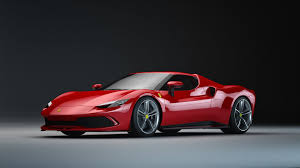
\includegraphics[width=\textwidth]{img/ferrari.jpg}};
                \node[align=center, fill=PrimaryColor, text=white, font=\bfseries, rounded corners=2pt, inner sep=4pt] 
                    at (2.5, 4.0) {Apache Spark RDDs};
            \end{tikzpicture}
        \end{column}

        \begin{column}{0.45\textwidth}
            \begin{itemize}
                \item \textbf{Hardware Evolution:} 
                \begin{itemize}
                    \item We use \textbf{Apache Spark RDDs}: the distributed ``Ferrari'' of in-memory computing.
                \end{itemize}
                \vspace{0.3cm}
                \item \textbf{The Bottleneck:} 
                \begin{itemize}
                    \item Legacy structures (Hash Trees) act like a \textbf{traffic jam} in a high-speed engine.
                \end{itemize}
            \end{itemize}
        \end{column}
    \end{columns}

    \vfill
    \begin{alertblock}{The Core Thesis}
        Infrastructure alone cannot solve $O(2^n)$. To exploit Spark's speed, we must replace ``Disk-era'' structures with memory-optimized \textbf{Tries}.
    \end{alertblock}
\end{frame}
